% Section 2.4:
\subsection{Objetivos de la Investigación}

\lipsum[7]

\subsubsection{Objetivo General}

\lipsum[8]

\subsubsection{Objetivos Específicos}

\lipsum[10]

\begin{figure}[ht]
  \caption{Figura con subfiguras}
  \label{fig:figura}
  \begin{subfigure}{0.35\textwidth}
      \centering
      \caption{A}
      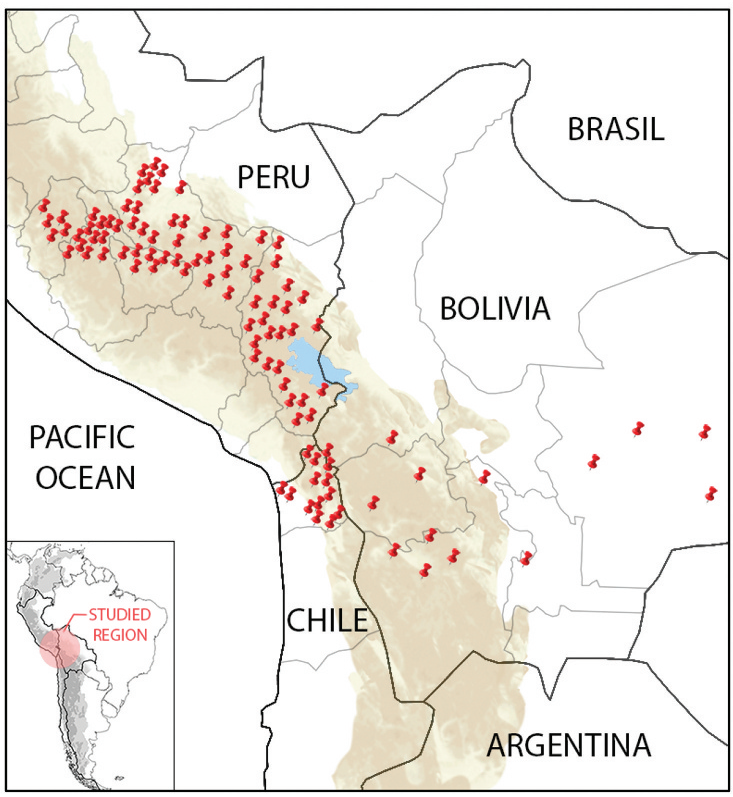
\includegraphics[scale=0.28]{F_Figures/11_Chapter II/Cap2_Imagen2a.png}
      \label{fig:subfig1}
  \end{subfigure}
  \hfill
  \begin{subfigure}{0.55\textwidth}
      \centering
      \caption{B}
      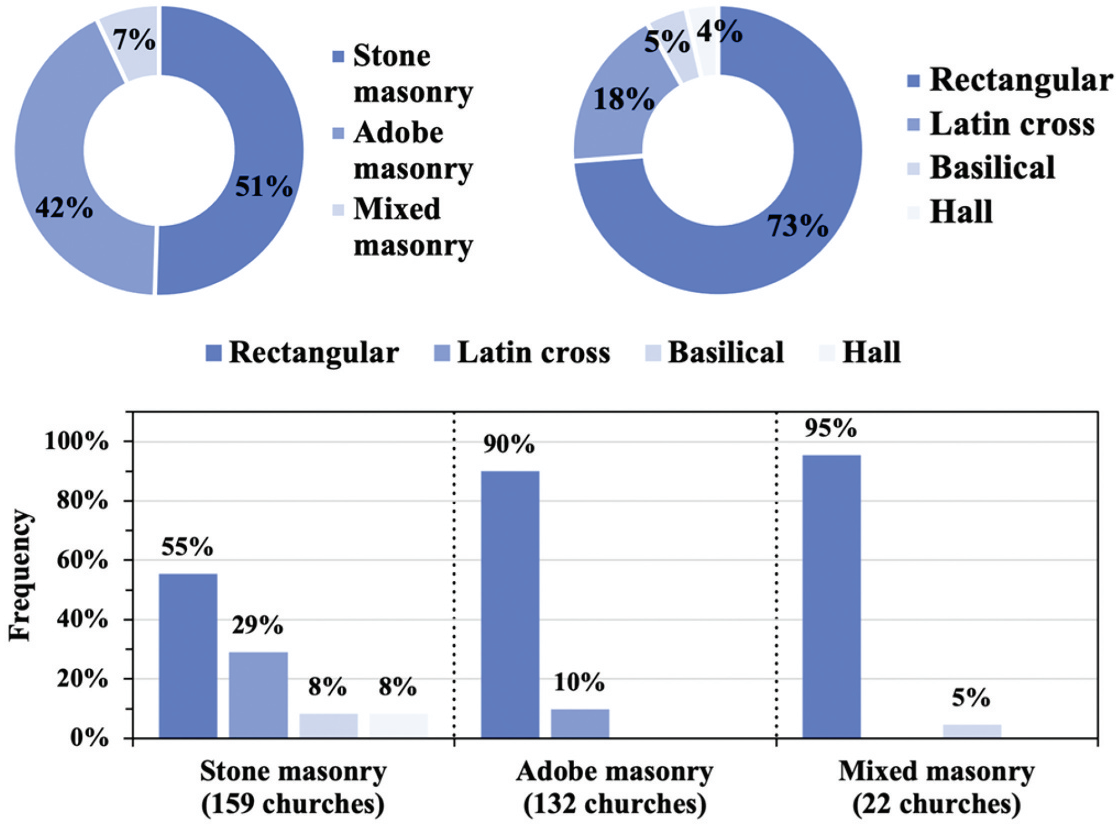
\includegraphics[scale=0.28]{F_Figures/11_Chapter II/Cap2_Imagen2b.png}
      \label{fig:subfig2}
  \end{subfigure}
  \figurenote{Buenas figuras}
\end{figure}

\subparagraph{Inter-rater reliability}
\lipsum[10]

\subparagraph{Test-retest reliability}
\lipsum[11]

\paragraph{Validity}
\lipsum[12]

\subparagraph{Face validity}
\lipsum[13]

\subparagraph{Construct validity}